              
                %% bare_jrnl.tex
%% V1.4b
%% 2015/08/26
%% by Michael Shell
%% see http://www.michaelshell.org/
%% for current contact information.
%%
%% This is a skeleton file demonstrating the use of IEEEtran.cls
%% (requires IEEEtran.cls version 1.8b or later) with an IEEE
%% journal paper.
%%
%% Support sites:
%% http://www.michaelshell.org/tex/ieeetran/
%% http://www.ctan.org/pkg/ieeetran
%% and
%% http://www.ieee.org/

%%*************************************************************************
%% Legal Notice:
%% This code is offered as-is without any warranty either expressed or
%% implied; without even the implied warranty of MERCHANTABILITY or
%% FITNESS FOR A PARTICULAR PURPOSE! 
%% User assumes all risk.
%% In no event shall the IEEE or any contributor to this code be liable for
%% any damages or losses, including, but not limited to, incidental,
%% consequential, or any other damages, resulting from the use or misuse
%% of any information contained here.
%%
%% All comments are the opinions of their respective authors and are not
%% necessarily endorsed by the IEEE.
%%
%% This work is distributed under the LaTeX Project Public License (LPPL)
%% ( http://www.latex-project.org/ ) version 1.3, and may be freely used,
%% distributed and modified. A copy of the LPPL, version 1.3, is included
%% in the base LaTeX documentation of all distributions of LaTeX released
%% 2003/12/01 or later.
%% Retain all contribution notices and credits.
%% ** Modified files should be clearly indicated as such, including  **
%% ** renaming them and changing author support contact information. **
%%*************************************************************************


% *** Authors should verify (and, if needed, correct) their LaTeX system  ***
% *** with the testflow diagnostic prior to trusting their LaTeX platform ***
% *** with production work. The IEEE's font choices and paper sizes can   ***
% *** trigger bugs that do not appear when using other class files.       ***                          ***
% The testflow support page is at:
% http://www.michaelshell.org/tex/testflow/


% Please refer to your journal's instructions for other
% options that should be set.
\documentclass[journal,onecolumn]{IEEEtran}
%
% If IEEEtran.cls has not been installed into the LaTeX system files,
% manually specify the path to it like:
% \documentclass[journal]{../sty/IEEEtran}





% Some very useful LaTeX packages include:
% (uncomment the ones you want to load)


% *** MISC UTILITY PACKAGES ***
%
%\usepackage{ifpdf}
% Heiko Oberdiek's ifpdf.sty is very useful if you need conditional
% compilation based on whether the output is pdf or dvi.
% usage:
% \ifpdf
%   % pdf code
% \else
%   % dvi code
% \fi
% The latest version of ifpdf.sty can be obtained from:
% http://www.ctan.org/pkg/ifpdf
% Also, note that IEEEtran.cls V1.7 and later provides a builtin
% \ifCLASSINFOpdf conditional that works the same way.
% When switching from latex to pdflatex and vice-versa, the compiler may
% have to be run twice to clear warning/error messages.






% *** CITATION PACKAGES ***
%
%\usepackage{cite}
% cite.sty was written by Donald Arseneau
% V1.6 and later of IEEEtran pre-defines the format of the cite.sty package
% \cite{} output to follow that of the IEEE. Loading the cite package will
% result in citation numbers being automatically sorted and properly
% "compressed/ranged". e.g., [1], [9], [2], [7], [5], [6] without using
% cite.sty will become [1], [2], [5]--[7], [9] using cite.sty. cite.sty's
% \cite will automatically add leading space, if needed. Use cite.sty's
% noadjust option (cite.sty V3.8 and later) if you want to turn this off
% such as if a citation ever needs to be enclosed in parenthesis.
% cite.sty is already installed on most LaTeX systems. Be sure and use
% version 5.0 (2009-03-20) and later if using hyperref.sty.
% The latest version can be obtained at:
% http://www.ctan.org/pkg/cite
% The documentation is contained in the cite.sty file itself.






% *** GRAPHICS RELATED PACKAGES ***
%
\ifCLASSINFOpdf
  \usepackage[pdftex]{graphicx}
  % declare the path(s) where your graphic files are
  % \graphicspath{{../pdf/}{../jpeg/}}
  % and their extensions so you won't have to specify these with
  % every instance of \includegraphics
  % \DeclareGraphicsExtensions{.pdf,.jpeg,.png}
\else
  % or other class option (dvipsone, dvipdf, if not using dvips). graphicx
  % will default to the driver specified in the system graphics.cfg if no
  % driver is specified.
  % \usepackage[dvips]{graphicx}
  % declare the path(s) where your graphic files are
  % \graphicspath{{../eps/}}
  % and their extensions so you won't have to specify these with
  % every instance of \includegraphics
  % \DeclareGraphicsExtensions{.eps}
\fi
% graphicx was written by David Carlisle and Sebastian Rahtz. It is
% required if you want graphics, photos, etc. graphicx.sty is already
% installed on most LaTeX systems. The latest version and documentation
% can be obtained at: 
% http://www.ctan.org/pkg/graphicx
% Another good source of documentation is "Using Imported Graphics in
% LaTeX2e" by Keith Reckdahl which can be found at:
% http://www.ctan.org/pkg/epslatex
%
% latex, and pdflatex in dvi mode, support graphics in encapsulated
% postscript (.eps) format. pdflatex in pdf mode supports graphics
% in .pdf, .jpeg, .png and .mps (metapost) formats. Users should ensure
% that all non-photo figures use a vector format (.eps, .pdf, .mps) and
% not a bitmapped formats (.jpeg, .png). The IEEE frowns on bitmapped formats
% which can result in "jaggedy"/blurry rendering of lines and letters as
% well as large increases in file sizes.
%
% You can find documentation about the pdfTeX application at:
% http://www.tug.org/applications/pdftex





% *** MATH PACKAGES ***
%
%\usepackage{amsmath}
% A popular package from the American Mathematical Society that provides
% many useful and powerful commands for dealing with mathematics.
%
% Note that the amsmath package sets \interdisplaylinepenalty to 10000
% thus preventing page breaks from occurring within multiline equations. Use:
%\interdisplaylinepenalty=2500
% after loading amsmath to restore such page breaks as IEEEtran.cls normally
% does. amsmath.sty is already installed on most LaTeX systems. The latest
% version and documentation can be obtained at:
% http://www.ctan.org/pkg/amsmath





% *** SPECIALIZED LIST PACKAGES ***
%
%\usepackage{algorithmic}
% algorithmic.sty was written by Peter Williams and Rogerio Brito.
% This package provides an algorithmic environment fo describing algorithms.
% You can use the algorithmic environment in-text or within a figure
% environment to provide for a floating algorithm. Do NOT use the algorithm
% floating environment provided by algorithm.sty (by the same authors) or
% algorithm2e.sty (by Christophe Fiorio) as the IEEE does not use dedicated
% algorithm float types and packages that provide these will not provide
% correct IEEE style captions. The latest version and documentation of
% algorithmic.sty can be obtained at:
% http://www.ctan.org/pkg/algorithms
% Also of interest may be the (relatively newer and more customizable)
% algorithmicx.sty package by Szasz Janos:
% http://www.ctan.org/pkg/algorithmicx




% *** ALIGNMENT PACKAGES ***
%
%\usepackage{array}
% Frank Mittelbach's and David Carlisle's array.sty patches and improves
% the standard LaTeX2e array and tabular environments to provide better
% appearance and additional user controls. As the default LaTeX2e table
% generation code is lacking to the point of almost being broken with
% respect to the quality of the end results, all users are strongly
% advised to use an enhanced (at the very least that provided by array.sty)
% set of table tools. array.sty is already installed on most systems. The
% latest version and documentation can be obtained at:
% http://www.ctan.org/pkg/array


% IEEEtran contains the IEEEeqnarray family of commands that can be used to
% generate multiline equations as well as matrices, tables, etc., of high
% quality.




% *** SUBFIGURE PACKAGES ***
%\ifCLASSOPTIONcompsoc
%  \usepackage[caption=false,font=normalsize,labelfont=sf,textfont=sf]{subfig}
%\else
%  \usepackage[caption=false,font=footnotesize]{subfig}
%\fi
% subfig.sty, written by Steven Douglas Cochran, is the modern replacement
% for subfigure.sty, the latter of which is no longer maintained and is
% incompatible with some LaTeX packages including fixltx2e. However,
% subfig.sty requires and automatically loads Axel Sommerfeldt's caption.sty
% which will override IEEEtran.cls' handling of captions and this will result
% in non-IEEE style figure/table captions. To prevent this problem, be sure
% and invoke subfig.sty's "caption=false" package option (available since
% subfig.sty version 1.3, 2005/06/28) as this is will preserve IEEEtran.cls
% handling of captions.
% Note that the Computer Society format requires a larger sans serif font
% than the serif footnote size font used in traditional IEEE formatting
% and thus the need to invoke different subfig.sty package options depending
% on whether compsoc mode has been enabled.
%
% The latest version and documentation of subfig.sty can be obtained at:
% http://www.ctan.org/pkg/subfig




% *** FLOAT PACKAGES ***
%
%\usepackage{fixltx2e}
% fixltx2e, the successor to the earlier fix2col.sty, was written by
% Frank Mittelbach and David Carlisle. This package corrects a few problems
% in the LaTeX2e kernel, the most notable of which is that in current
% LaTeX2e releases, the ordering of single and double column floats is not
% guaranteed to be preserved. Thus, an unpatched LaTeX2e can allow a
% single column figure to be placed prior to an earlier double column
% figure.
% Be aware that LaTeX2e kernels dated 2015 and later have fixltx2e.sty's
% corrections already built into the system in which case a warning will
% be issued if an attempt is made to load fixltx2e.sty as it is no longer
% needed.
% The latest version and documentation can be found at:
% http://www.ctan.org/pkg/fixltx2e


%\usepackage{stfloats}
% stfloats.sty was written by Sigitas Tolusis. This package gives LaTeX2e
% the ability to do double column floats at the bottom of the page as well
% as the top. (e.g., "\begin{figure*}[!b]" is not normally possible in
% LaTeX2e). It also provides a command:
%\fnbelowfloat
% to enable the placement of footnotes below bottom floats (the standard
% LaTeX2e kernel puts them above bottom floats). This is an invasive package
% which rewrites many portions of the LaTeX2e float routines. It may not work
% with other packages that modify the LaTeX2e float routines. The latest
% version and documentation can be obtained at:
% http://www.ctan.org/pkg/stfloats
% Do not use the stfloats baselinefloat ability as the IEEE does not allow
% \baselineskip to stretch. Authors submitting work to the IEEE should note
% that the IEEE rarely uses double column equations and that authors should try
% to avoid such use. Do not be tempted to use the cuted.sty or midfloat.sty
% packages (also by Sigitas Tolusis) as the IEEE does not format its papers in
% such ways.
% Do not attempt to use stfloats with fixltx2e as they are incompatible.
% Instead, use Morten Hogholm'a dblfloatfix which combines the features
% of both fixltx2e and stfloats:
%
% \usepackage{dblfloatfix}
% The latest version can be found at:
% http://www.ctan.org/pkg/dblfloatfix




%\ifCLASSOPTIONcaptionsoff
%  \usepackage[nomarkers]{endfloat}
% \let\MYoriglatexcaption\caption
% \renewcommand{\caption}[2][\relax]{\MYoriglatexcaption[#2]{#2}}
%\fi
% endfloat.sty was written by James Darrell McCauley, Jeff Goldberg and 
% Axel Sommerfeldt. This package may be useful when used in conjunction with 
% IEEEtran.cls'  captionsoff option. Some IEEE journals/societies require that
% submissions have lists of figures/tables at the end of the paper and that
% figures/tables without any captions are placed on a page by themselves at
% the end of the document. If needed, the draftcls IEEEtran class option or
% \CLASSINPUTbaselinestretch interface can be used to increase the line
% spacing as well. Be sure and use the nomarkers option of endfloat to
% prevent endfloat from "marking" where the figures would have been placed
% in the text. The two hack lines of code above are a slight modification of
% that suggested by in the endfloat docs (section 8.4.1) to ensure that
% the full captions always appear in the list of figures/tables - even if
% the user used the short optional argument of \caption[]{}.
% IEEE papers do not typically make use of \caption[]'s optional argument,
% so this should not be an issue. A similar trick can be used to disable
% captions of packages such as subfig.sty that lack options to turn off
% the subcaptions:
% For subfig.sty:
% \let\MYorigsubfloat\subfloat
% \renewcommand{\subfloat}[2][\relax]{\MYorigsubfloat[]{#2}}
% However, the above trick will not work if both optional arguments of
% the \subfloat command are used. Furthermore, there needs to be a
% description of each subfigure *somewhere* and endfloat does not add
% subfigure captions to its list of figures. Thus, the best approach is to
% avoid the use of subfigure captions (many IEEE journals avoid them anyway)
% and instead reference/explain all the subfigures within the main caption.
% The latest version of endfloat.sty and its documentation can obtained at:
% http://www.ctan.org/pkg/endfloat
%
% The IEEEtran \ifCLASSOPTIONcaptionsoff conditional can also be used
% later in the document, say, to conditionally put the References on a 
% page by themselves.




% *** PDF, URL AND HYPERLINK PACKAGES ***
%
%\usepackage{url}
% url.sty was written by Donald Arseneau. It provides better support for
% handling and breaking URLs. url.sty is already installed on most LaTeX
% systems. The latest version and documentation can be obtained at:
% http://www.ctan.org/pkg/url
% Basically, \url{my_url_here}.




% *** Do not adjust lengths that control margins, column widths, etc. ***
% *** Do not use packages that alter fonts (such as pslatex).         ***
% There should be no need to do such things with IEEEtran.cls V1.6 and later.
% (Unless specifically asked to do so by the journal or conference you plan
% to submit to, of course. )


% correct bad hyphenation here
\hyphenation{op-tical net-works semi-conduc-tor}


\begin{document}

% Title
\title{CSE 578: Data Visualization - Course Project}

% Author
\author{Andrey Sokolov}

\maketitle

\begin{abstract}
    This report presents an in-depth analysis of income-related factors to develop a
    marketing profile for UVW College. As part of our role at XYZ Data Company, we
    explored a dataset derived from the US Census Bureau, examining how various
    demographic and economic attributes influence whether an individual earns more than \$50,000 annually. 
    
    A comprehensive data pipeline was implemented, including data cleaning, feature
    selection, encoding techniques, and correlation analysis to identify the most
    impactful variables. Hierarchical clustering and principal component analysis
    (PCA) were utilized to reduce dimensionality and uncover hidden patterns.
    Multiple visualization techniques—such as stacked bar charts, heatmaps, and hierarchical clustering dendrograms—were applied to highlight key trends and relationships.
    
    Our findings indicate that factors such as marital status, occupation,
    education level, and hours worked per week exhibit the strongest correlations
    with income. Negative correlations with attributes like "relationship" and
    "sex" suggest structural influences that warrant further exploration.
    We also compared different classification models, evaluating decision trees,
    support vector machines (SVM), and neural networks for their predictive accuracy in income classification.
    
    The results of this study will inform UVW College’s enrollment and marketing strategies,
    allowing for data-driven decision-making. Future work includes refining predictive models,
    integrating additional socioeconomic data, and developing interactive visual tools to enhance usability for stakeholders.
    \end{abstract}

\section{Introduction}
XYZ Data Company is conducting an income-based analysis for UVW College to develop
a targeted marketing profile. The objective is to explore the influence of various
socioeconomic factors on an individual’s income level, specifically determining
whether they earn more or less than 50,000USD per year.

This analysis leverages data from the U.S. Census Bureau, including key attributes
such as education, occupation, marital status, and work hours per week. Through
data-driven visualizations and predictive modeling, this project aims to uncover
meaningful insights that will inform UVW College’s marketing and enrollment strategies.
By identifying trends and relationships between demographic characteristics and income,
we aim to help UVW College optimize its outreach efforts and target prospective
students more effectively.



\section{Data Acquisition and Preprocessing}


\subsection{Data Cleaning Approach}
One of the initial challenges was ensuring the dataset was clean and structured correctly. The dataset contained missing values, inconsistencies in categorical variables, and redundant features. The steps taken were:
\begin{itemize}
    \item Removed 'fnlwgt' from DataFrame as it will not be used
    \item Identified and removed leading/trailing whitespace characters in multiple columns, identified by isolating unique values
    \item Checked for minimum and maximum of all continuous variables as well as any negative values. There are two maximums that seem to be capped - capital-gain(99999) and hours-per-week(99)
    \item Also identified missing values in the data, marked as '?'. These were replaced with 'None' as an indicator of missing values for Python interpretation
    \item Noted - number of missing values is quite low and only for a few variables - workclass and occuption(a correlated number) and native-country
\end{itemize}

\section{Feature Selection and Engineering}

\begin{description}
    \item[Q:] \textbf{Which attributes should be prioritized for analysis? How should they be chosen?}
    \item[A:] Initially, attribute selection was based on intuition and cursory data exploration. However, to ensure an evidence-based approach, correlation analysis and feature importance techniques should be applied. Attributes with strong correlations to income can be refined from preliminary machine learning models or manual EDA.

    \item[Q:] \textbf{What is the best algorithm to classify/model this kind of data? Decision Tree vs. SVM vs. Neural Network?}
    \item[A:] Several machine learning algorithms were considered and researched. A Decision Tree model seems like a good fit because it offers interpretability and handles categorical data well.

\end{description}

\section{Exploratory Data Analysis}

\subsection{Choosing the First Attributes for Analysis}
The first step in feature selection was identifying the most relevant attributes affecting income classification. The following approach was taken:
\begin{itemize}
    \item Conducted an initial exploratory data analysis to find at least one predictive attribute
    \item Selected \textbf{Education} as the primary attribute for early investigation, as it showed promising correlation with income level.
\end{itemize}

\subsection{Creating the First Visualization}
To validate early assumptions, the first visualization was created:
\begin{itemize}
    \item To plot salary versus education, we considered the binary nature of our key factor, salary. Since it is broken up into less than 50K and greater than 50K, it makes sense to plot using another attribute as an axis.
    \item Education is already broken up into integer values in the education-num category, but there are too many categories to comfortably display
    \item Therefore, we can consolidate the grade levels into one block, the non high school grad - this reduces down to 8 educational categories.
    \item Some thought was given to keeping associate degree (vocational) as "trade school", but outcomes are so similar to the traditional associate degree that it made more sense to combine the two
    \item Design Choices: Used distinct color coding for income categories, clear axis labeling, and a balanced layout for readability.
    \item Implementation: The visualization was created using Seaborn in Python.
    \item The aggregate visualization did a good job at representing the correlation between each education bracket and salary and clarity was further improved by sorting by education level left to right
\end{itemize}


\begin{figure}[t]
    \centering
    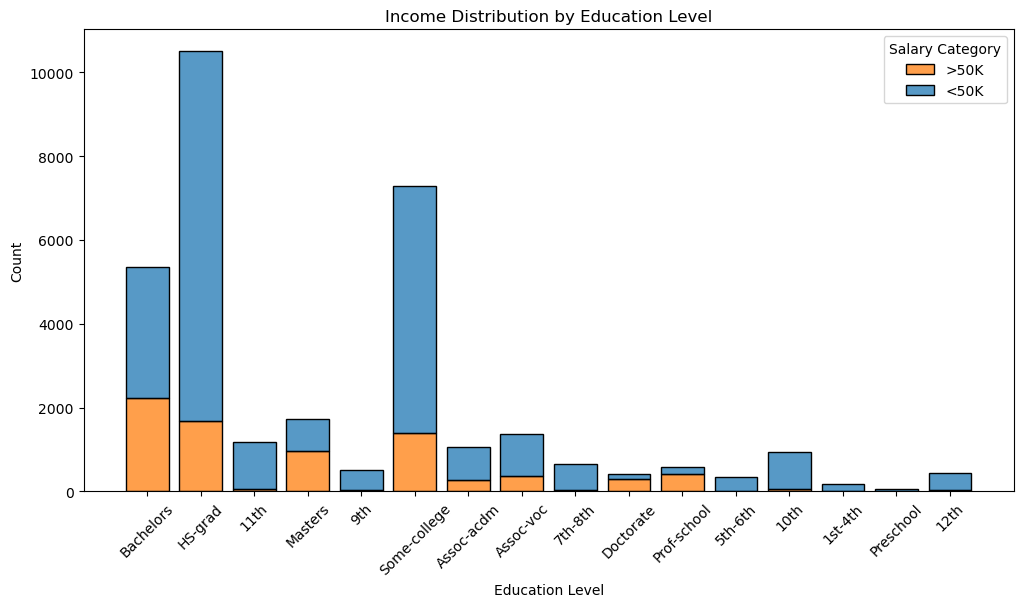
\includegraphics[width=0.9\linewidth]{hist_bad.png}  % Reduce width slightly
    \caption{Income vs Education without aggregates and ranked order}
    \label{fig:income_vs_education_no_agg}
\end{figure}

\begin{figure}[t]
    \centering
    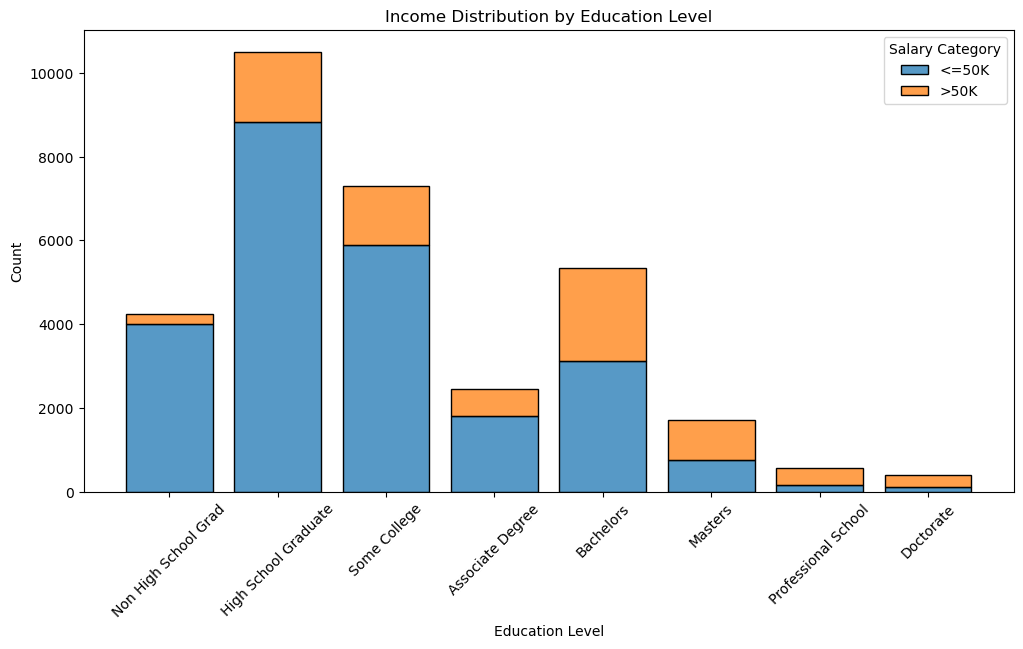
\includegraphics[width=0.9\linewidth]{hist_4.png}  % Reduce width slightly
    \caption{Final histogram for Income vs Education}
    \label{fig:final_income_vs_education}
\end{figure}
\section{Initial / Key Insights from Education Level vs. Income Distribution}

\begin{itemize}
    \item \textbf{Higher Education Correlates with Higher Income:} Individuals with advanced degrees (Masters, Professional School, Doctorate) have a significantly higher proportion of incomes above \$50K compared to those with lower educational attainment.
    
    \item \textbf{Most Common Education Levels:} The majority of individuals fall into the \textit{High School Graduate} and \textit{Some College} categories, making them the largest groups in the dataset. However, their income distributions do not show their education to be a predictor for the less than \$50K and greater than \$50K groups.
    
    \item \textbf{Education Alone is Not a Sole Predictor of Income:} Even at the Bachelor's level, a substantial number of individuals still earn less than \$50K. This suggests that additional factors such as work class, occupation, and experience must be considered to better predict income.
\end{itemize}


\section{User Stories}
To structure our approach further, we defined the following additional user stories that represent key stakeholders:

\subsection{User Story \#1}
\begin{itemize}
    \item \textbf{Role:} Director of the UVW marketing team
    \item \textbf{Goal:} To analyze how the combination of sex, marital-status, and age influences salary category.
    \item \textbf{Context/Insights:}
    \begin{itemize}
        \item Our findings suggest that marital status has one of the strongest correlations with income, particularly for married individuals.
        \item Age plays a crucial role in career progression, with mid-career individuals (40-50 years old) more likely to reach higher income brackets.
        \item There is a significant gender income gap, and this analysis will determine whether marital status and age mitigate or amplify this effect.
        \item Understanding these relationships will help UVW College craft targeted messaging for different demographics and optimize outreach strategies.
    \end{itemize}

\end{itemize}

\subsection{User Story \#1}
\begin{itemize}
    \item \textbf{Role:} Director of the UVW marketing team
    \item \textbf{Goal:} To analyze how the combination of occupation type, hours worked per week, and capital gains influences salary category.
\end{itemize}

\subsection{User Story \#2}
\begin{itemize}
    \item \textbf{Role:} Workforce development strategist
    \item \textbf{Goal:} To examine variations in income levels across different work classes and education levels.
\end{itemize}

\subsection{User Story \#3}
\begin{itemize}
    \item \textbf{Role:} Director of the UVW marketing team
    \item \textbf{Goal:} To identify the strongest predictors of high-income individuals.
\end{itemize}

\subsection{User Story \#4}
\begin{itemize}
    \item \textbf{Role:} UVW Policy analyst
    \item \textbf{Goal:} To assess whether marital status plays a significant role in salary levels across different age groups.
\end{itemize}

\subsection{User Story \#5}
\begin{itemize}
    \item \textbf{Role:} UVW Foreign relations researcher
    \item \textbf{Goal:} To compare income variations among individuals based on their native country and work class.
\end{itemize}


\section{Appendix}
\subsection{Setup}
\begin{enumerate}
    \item Latex set up for drafting submissions in VS Code for Mac by installing Mactex
    \item Started a Jupyter notebook server and began coding/using markdown to explain each data analysis step
    \item Installed and configured necessary Python libraries, including: 
    \texttt{pandas}, \texttt{seaborn}, \texttt{matplotlib}, and 
    \texttt{scikit-learn}.
    \item Set up Git version control to track code changes and manage different analysis iterations.
    \item Started a Jupyter notebook server and began coding and markdown to explain each data analysis step
    \item Documented key findings and insights in Jupyter notebooks for reference in the final report.
\end{enumerate}
\end{document}
